\documentclass{article}

\usepackage{graphicx}
\usepackage{tikz}
\usepackage{tikzsymbols}
\usetikzlibrary{calc,patterns,shapes.geometric}
\pagestyle{empty}
\usepackage[margin=0pt]{geometry}
\geometry{papersize={14in,12in}}

\def\centerarc[#1](#2)(#3:#4:#5){\draw[#1] ($(#2)+({#5*cos(#3)},{#5*sin(#3)})$) arc (#3:#4:#5);}

\begin{document}
	\begin{figure}
		\centering
		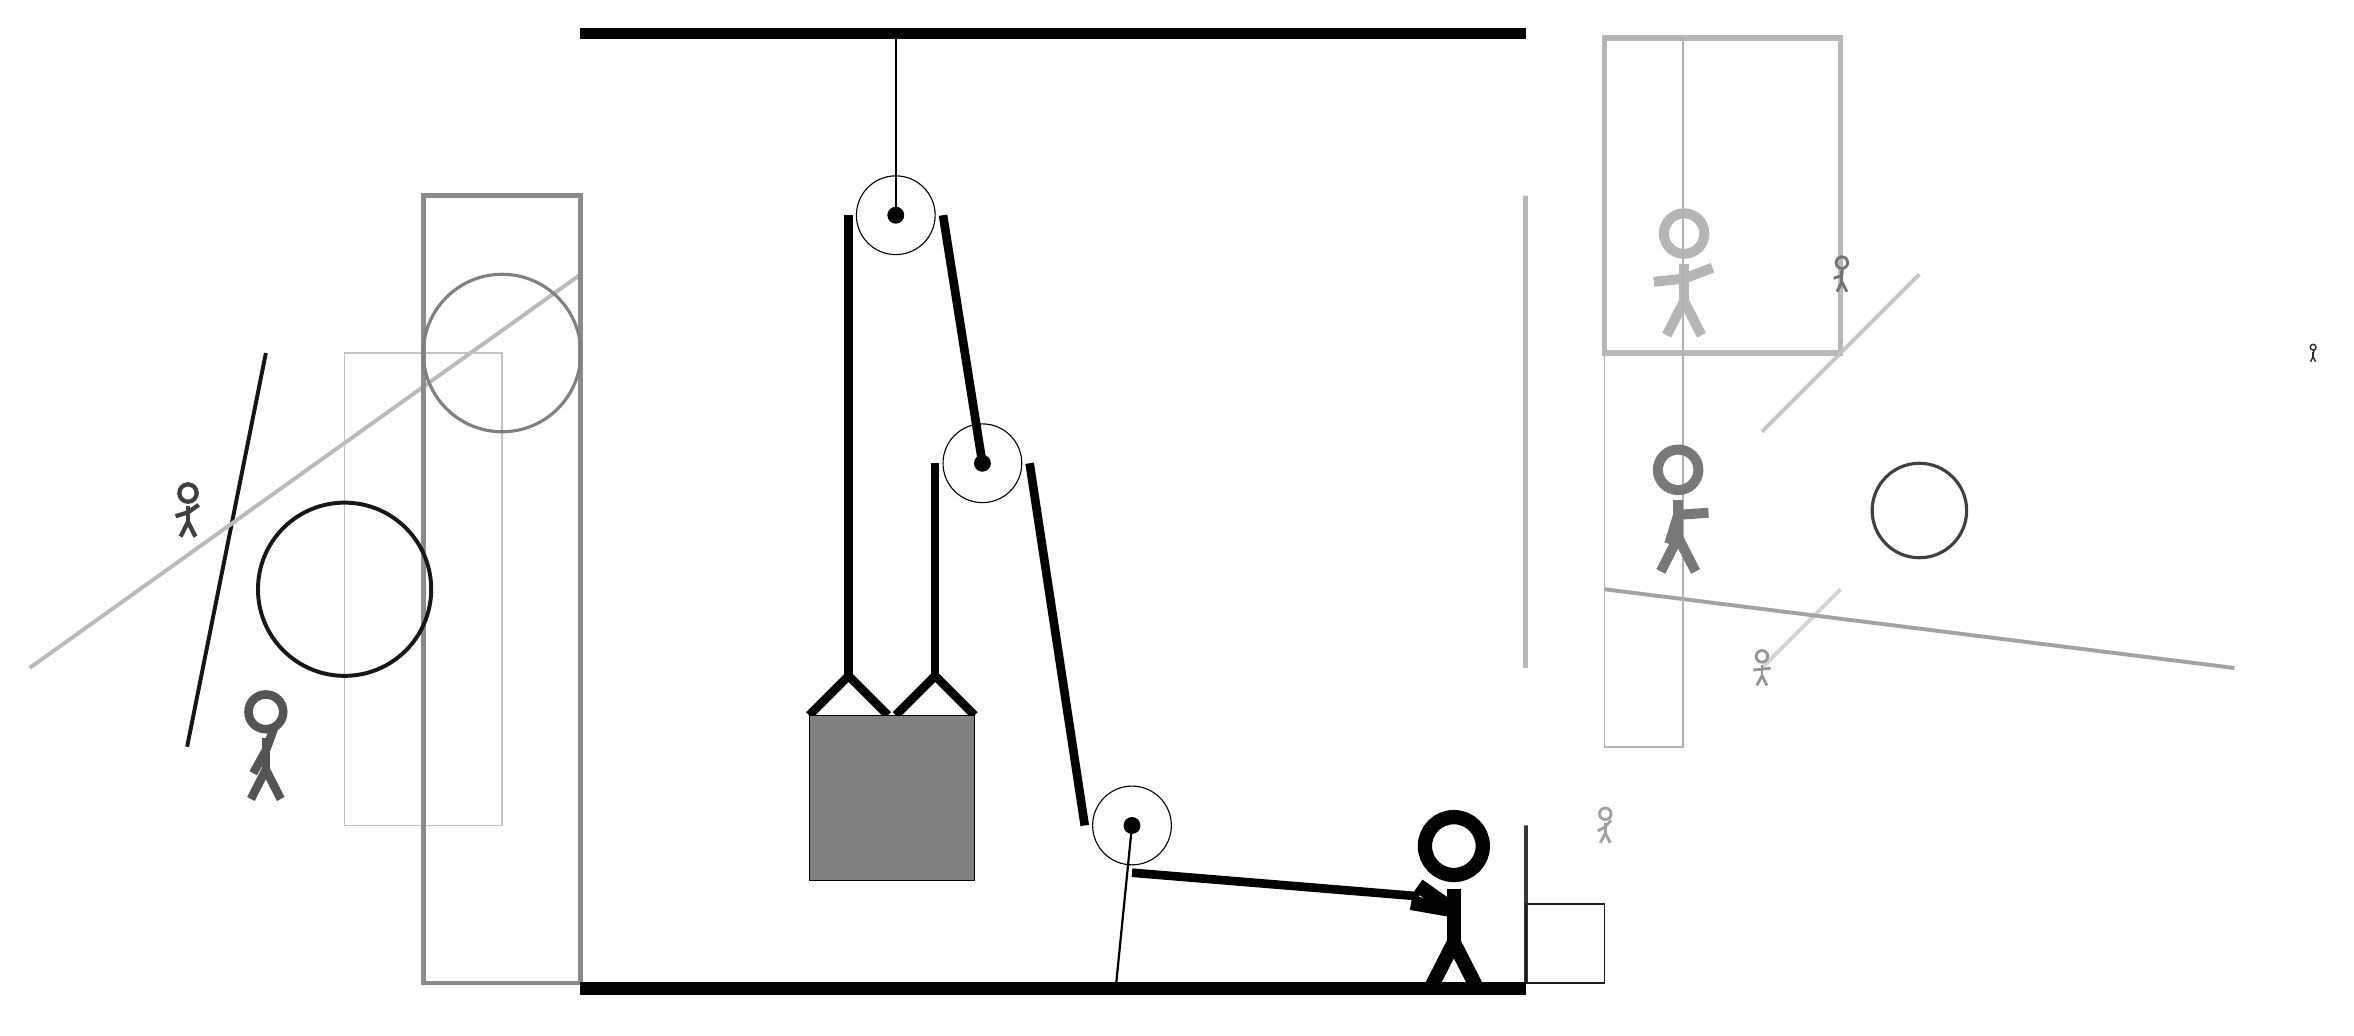
\begin{tikzpicture}
			%%%%% START %%%%%
			
			\draw[fill=black] (-2, 9) rectangle (10, 9.125);
			
			\draw (2, 6.75) circle (0.5);
			\draw[fill=black] (2, 6.75) circle (0.1);
			\draw[thick] (2, 6.75) -- (2, 9);
			
			\draw[line width=0.5mm, color=black!79] (10, -3) rectangle (10, -1);
			
			\draw [line width=0.4mm, color=black!75](15, 3) circle (0.6);
			\draw[line width=0.5mm, color=black!92](-6, 5) -- (-7, 0);
			\node[line width=0.5mm, color=black!67] at (-6, 0) {\Strichmaxerl[6][61][70]};
			
			\draw[line width=0.2mm, color=black!89] (10, -2) rectangle (11, -3);
			\draw[line width=0.4mm, color=black!100] (-2, -2) rectangle (-2, -1);
			\draw[line width=0.7mm, color=black!28] (11, 9) rectangle (14, 5);
			\draw[line width=0.5mm, color=black!27](-2, 6) -- (-9, 1);
			\draw[line width=0.2mm, color=black!24] (-3, -1) rectangle (-5, 5);
			
			\draw[line width=0.6mm, color=black!46] (-2, -3) rectangle (-4, 7);
			\node[line width=0.3mm, color=black!55] at (14, 6) {\Strichmaxerl[2][18][86]};
			
			\draw[line width=0.5mm, color=black!17](13, 1) -- (14, 2);
			\draw[line width=0.5mm, color=black!36](11, 2) -- (19, 1);
			
			\node[line width=0.5mm, color=black!75] at (-7, 3) {\Strichmaxerl[3][17][35]};
			\node[line width=0.6mm, color=black!29] at (12, 6) {\Strichmaxerl[7][6][21]};
			\draw [line width=0.5mm, color=black!91](-5, 2) circle (1.1);
			
			\draw[line width=0.2mm, color=black!31] (11, 9) rectangle (12, 0);
			\node[line width=0.5mm, color=black!83] at (20, 5) {\Strichmaxerl[1][89][74]};
			\draw [line width=0.4mm, color=black!50](-3, 5) circle (1.0);
			
			\node[line width=0.7mm, color=black!53] at (12, 3) {\Strichmaxerl[7][73][4]};
			\node[line width=0.6mm, color=black!41] at (13, 1) {\Strichmaxerl[2][5][7]};
			
			\draw[line width=0.5mm, color=black!23](15, 6) -- (13, 4);
			\node[line width=0.2mm, color=black!37] at (11, -1) {\Strichmaxerl[2][30][48]};
			\draw[line width=0.6mm, color=black!28] (10, 7) rectangle (10, 1);
			
			\draw (3.1, 3.6) circle (0.5);
			\draw[fill=black] (3.1, 3.6) circle (0.1);
			
			\draw (5, -1) circle (0.5);
			\draw[fill=black] (5, -1) circle (0.1);
			\draw[thick] (5, -1) -- (4.8, -3);
			
			\draw[line width = 1.1mm]  (0.9, 0.4) -- (1.4, 0.9) -- (1.9, 0.4);
			\draw[line width = 1.1mm]  (2.0, 0.4) -- (2.5, 0.9) -- (3.0, 0.4);
			\draw[fill=black!50] (0.9, 0.4) rectangle (3.0, -1.7);
			
			\draw[line width = 1.1mm] (1.4, 6.75) -- (1.4, 0.9);
			\centerarc[line width = 1.1mm](2, 6.75)(0:180:0.6);
			\draw[line width = 1.1mm] (2.6, 6.75) -- (3.1, 3.6);
			\draw[line width = 1.1mm] (2.5, 3.6) -- (2.5, 0.9);
			\centerarc[line width = 1.1mm](3.1, 3.6)(0:180:0.6);
			\draw[line width = 1.1mm] (3.7, 3.6) -- (4.4, -1);
			\centerarc[line width = 1.1mm](5, -1)(180:270:0.6);
			\draw[line width = 1.1mm] (5, -1.6) -- (8.65, -1.9);
			
			\node at (9, -2) {\Strichmaxerl[10][-35][170]};
			
			\draw[fill=black] (-2, -3) rectangle (10, -3.15);
			
			%%%%% END %%%%%
		\end{tikzpicture}
	\end{figure}	
\end{document}